\documentclass[11pt, a4paper, notitlepage]{report}
\usepackage[dvips]{graphicx,color,rotating}
\usepackage{polski}
\usepackage[utf8]{inputenc}
\usepackage{pstricks}
\usepackage{lipsum}
\usepackage{titling}
\usepackage{appendix}
\usepackage[euler]{textgreek}
\usepackage{amsmath}
\usepackage{listings}

\pretitle{
	\begin{center} 
		
\includegraphics[width=40pt,height=40pt]{graphics/znak_pk} \\ 
		 \Huge\bfseries}
\posttitle{\par\end{center}\vskip 0.5em}
\preauthor{\begin{center} \Large  KWD  \\  \LARGE\ttfamily}
\postauthor{ \end{center}}
\predate{\par\large\centering}
\postdate{\par}

\pagestyle{headings}


\author{
  Dominik Tamiołło \\
  Sebastian Smulski
}

\title{\textbf{Neuronowy model dawcy krwi}}
\date{27.01.2021}

\pagenumbering{roman} 

\begin{document}++++
\clearpage\maketitle
\thispagestyle{empty}
\begin{abstract}
	Projekt przedstawia model za pomocą którego jesteśmy w stanie stwierdzić czy określony dawca został dopuszczony do oddania krwi. Jest to typowy problem klasyfikacji binarnej. Wspomaganie procesu decyzyjnego modelu zostało zrealizowane przy pomocy regresji logistycznej. Dane do uczenia modelu zostały pobrane z repozytorium uczelni Donald Bren School of Information \& Computer Sciences
\end{abstract}

\clearpage \tableofcontents
\thispagestyle{empty}

\setcounter{page}{1}

\chapter{Wprowadzenie}
\pagenumbering{arabic}

Projekt przedstawia model za pomocą którego jesteśmy w stanie stwierdzić czy określony dawca został dopuszczony do oddania krwi. Dane do uczenia modelu zostały pobrane z repozytorium uczelni Donald Bren School of Information \& Computer Sciences. Przejdźmy do analizy danych.
Zbiór danych składa się z 748 rekordów zawierających następujące pola : \\
\begin{enumerate}  
\item Recency - ilość miesięcy ile upłynęło od ostatniego oddania krwi. 
\item Frequency - totalna liczba donacji.
\item Monetary - ilość oddanej krwi z milimetrach sześciennych.
\item Time - ilość miesięcy od pierwszej donacji krwi.
\item Wartość binarna oznaczająca czy dawca oddał krew w marcu 2007 roku.
\end{enumerate}
\newpage
Podział dawców na osoby które oddały krew (wartość 1) oraz które nie oddały (wartość 0) \\
\begin{figure}[h!]
  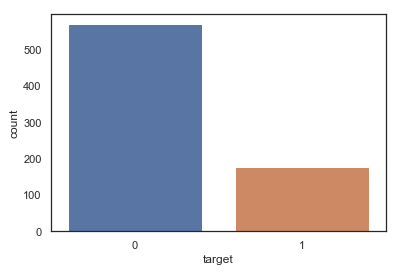
\includegraphics[width=300pt,height=40pt]{graphics/sns}
  \caption{Ilościowy podział osób oddających krew}
  \label{fig:scale}
\end{figure}
Odpowiednio 178 osób oddało krew a 570 nie oddało. \\
Wartości nie są zbalansowane co może zaowocować nie najlepszymi wynikami. Najlepszą sytuacją dla trenowania modelu byłyby dane o równej ilości wartości zer oraz jedynek. Uczenie maszynowe w problemie klasyfikacji daje najbardziej wiarygodne rezultaty gdy jest w stanie "zobaczyć" podobną ilość wyników pozytywnych jak i negatywnych.
\section{Opis problemu}
Na podstawie danych które otrzymaliśmy w naszym zbiorze postaramy się określić czy dana osoba została dawcą krwi. Przed każdym oddaniem krwi potencjalny dawca przechodzi odpowiednie badania kwalifikacyjne, pobranie krwi w celu sprawdzenia poziomu hemoglobiny oraz wywiad z lekarzem. Nasz model może być dodatkowo wykorzystany do wspomagania decyzji w określeniu czy dany kandydat może być odpowiednim dawcą. W tym celu będziemy nauczać model uczenia maszynowego przy wykorzystaniu regresji logistycznej z wykorzystaniem bibliotek 

\begin{enumerate}  
\item sklearn 
\item pandas
\item tpot
\item numpy
\item sns
\end{enumerate}

Zbiór zostanie odpowiednio podzielony na podzbiory trenujące oraz testowe w proporcji 75:25.
Dane testowe nie będą wcale trenowane, posłużą one nam w celu weryfikacji jakości naszego modelu. Wybraną przez nas metodą uczenia nadzorowanego została regresja logistyczna którą poznaliśmy już na zajęciach laboratoryjnych. Nasz wybór został umotywowany poprzez analizę zbioru danych. W celu weryfikacji decyzji skorzystaliśmy z biblioteki TPOT która poprzez programowanie genetyczne próbuje ustalić najlepszą metodę uczenia oraz parametry dodatkowe. \\
Dane otrzymane przez nas są nieustandaryzowane, to znaczy, ich wartości różnią się od siebie o kilka rzędów wartości. \\

\begin{figure}[h!]
  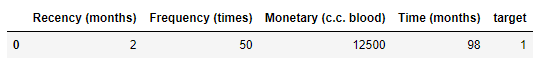
\includegraphics[width=300pt,height=40pt]{graphics/scale}
  \caption{Rekord danych}
  \label{fig:scale}
\end{figure}
Zmienne, które są mierzone w różnych skalach, nie wpływają w równym stopniu na dopasowanie modelu i wyuczoną funkcję modelu i mogą w końcu spowodować powstanie błędu. Przed uczeniem poddaliśmy je ustandaryzowaniu do wartości tego samego rzędu.

Mając odpowiednie dane do trenowania modelu jesteśmy w stanie przystąpić do implementowania projektu, który jest typowym problemem klasyfikacji binarnej.

\chapter{Opis metody}
\section{Wprowadzenie teoretyczne}
Regresja logistyczna to uczenie nadzorowane. Zakłada ona, że dane mogą być rozdzielone poprzez linię lub płaszczyznę n-wymiarową. Oznacza że jest to modele liniowy. Klasyfikacja odbywa się poprzez wyliczenie wartości wielomianu pierwszego stopnia w postaci


$$ y =\omega 1 * x1+ \omega 2 * x2+… + \omega n* xn $$ \\
gdzie, \\
x - dana wejściowa \\
\textomega \, - waga tego parametru \\
n - ilość parametrów wejściowych. \\
\\
Kolejnym krokiem jest podstawienie uzyskanego wyniku do funkcji logistycznej (dla przykładu sigmoid bądź tanh), w celu uzyskania wartości binarnej. Po uzyskaniu jednej z dwóch wartości jesteśmy w stanie zaklasyfikować daną wejściową do pierwszej bądź drugiej grupy. Podział odbywa się na przestrzeni jeżeli:
$$ y >= 0.5 $$ wtedy klasa pierwsza, w przeciwnym wypadku klasa druga.
\\
\\
Proces uczenia maszynowego polega na takim doborze wag \textomega, aby uzyskać na zbiorze uczącym jak największy odsetek poprawnych klasyfikacji. Uzyskuje się to poprzez wyliczenie funkcji kosztu oraz jej minimalizację z wykorzystaniem algorytmu gradientu prostego. 
\newpage
\begin{figure}[h!]
  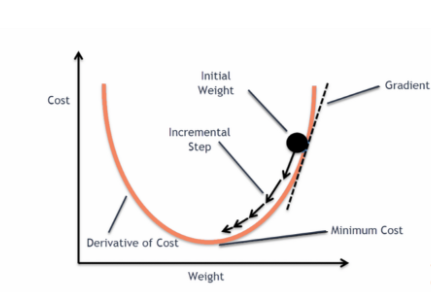
\includegraphics[scale=1]{graphics/gradient}
  \caption{Gradient prosty}
  \label{fig:gradient}
\end{figure}

W regresji logistycznej staramy się stworzyć taki podział, który rozgraniczy obiekty na dwie grupy jak zaprezentowane na obrazku poniżej.

\begin{figure}[h!]
  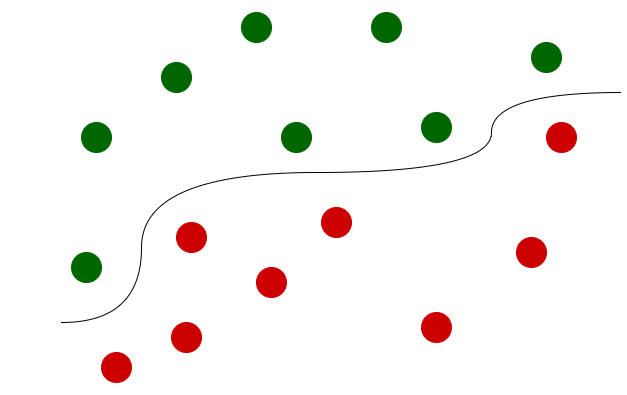
\includegraphics[scale=0.5]{graphics/logistic}
  \caption{Wizualizacja danych dla problemu dwuwymiarowego}
  \label{fig:gradient}
\end{figure}
\newpage

\section{Badania symulacyjne}
Przed przystąpieniem do trenowania modelu sprawdziliśmy jakość naszych danych poprzez narzędzia statystyczne. Na wykresie poniżej przedstawiliśmy rozkład zmiennych oraz ich zależności pomiędzy sobą. Widać że dane na przekątnej niekoniecznie odzwierciedlają rozkład normalny, co będzie miało wpływ na jakość naszego modelu. Oznacza to że dane otrzymane przez nas nie są idealne.

 \begin{figure}[h!]
  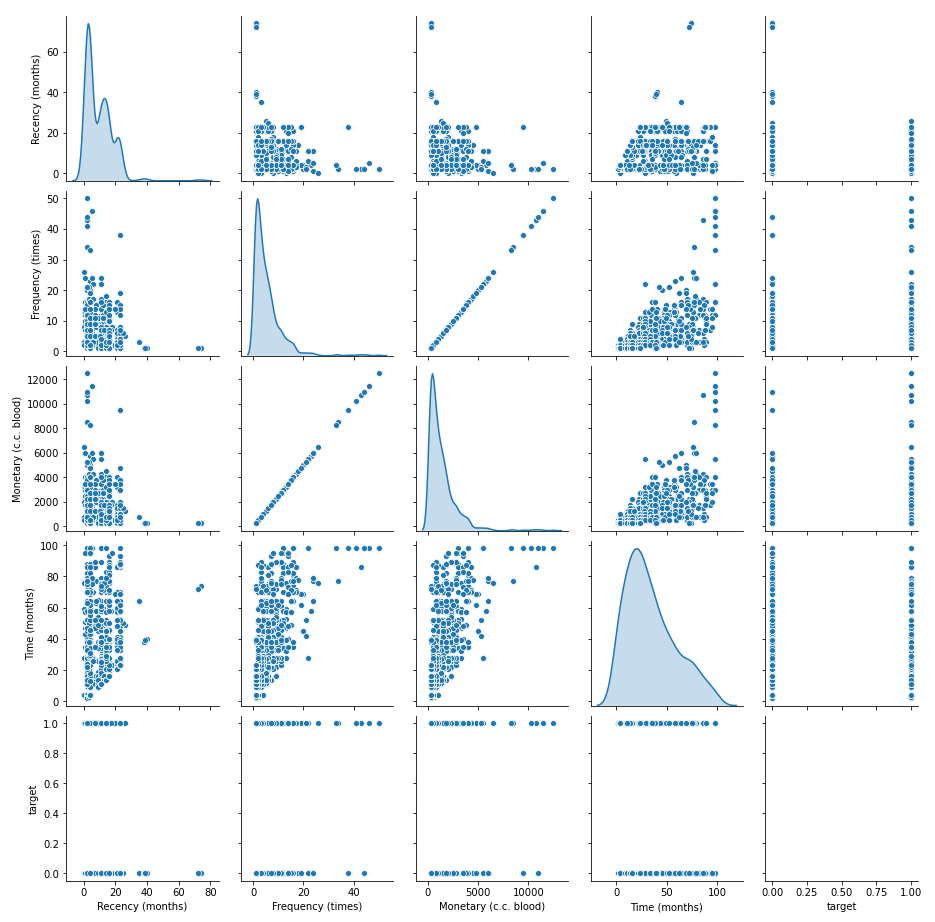
\includegraphics[scale=0.5]{graphics/distribution}
  \caption{Wizualizacja rozkładu zmiennych}
  \label{fig:distribution}
\end{figure}

\newpage
Następnie po wytrenowaniu naszego modelu sprawdziliśmy czy nasz model jest w stanie wiarygodnie przewidzieć wynik na podstawie danych testowych. Sprawdziliśmy dla pacjenta (którego parametrów nasz model wcześniej nie "widział") nr 41.  

 \begin{figure}[h!]
  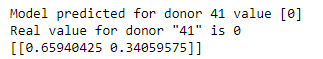
\includegraphics[scale=1]{graphics/predict}
  \caption{Wynik predykcji danych testowych}
  \label{fig:predict}
\end{figure}

Wynik jest poprawny oraz został wybrany z prawdopodobieństwem 0.66 (trzecia linijka)
W ogólności nasz model przewidział poprawnie w 78 \% przypadków (model accuracy), a jego macierz konfuzji wygląda następująco.

\[
M=
  \begin{bmatrix}
    142 & 1\\
    40 & 4 
  \end{bmatrix}
\]
Widać wyraźnie że model dobrze przewiduje jeden stan ale z drugim sobie nie radzi. Może to wynikać z wcześniej wymienionej dysproporcji w podziale wyników pozytywnych i negatywnych jak również złej dystrybucji danych.
Przeprowadziliśmy również sprawdzenie krzyżowe dające szerszy obraz na to czy model spełnia nasze wymagania. Podzieliliśmy zbiór na 6 osobnych części i ich poprawności umieściliśmy w macierzy poniżej

\[
  \begin{bmatrix}
    0.8 & 0.76 & 0.752 & 0.776 & 0.8064 & 0.7661
  \end{bmatrix}
\]
Możemy zauważyć że są to wyniki podobne do jakości ogólnej modelu. Dla każdej porcji danych jakość modelu jest bardzo podobna. Wnioskujemy że model został wytrenowany dobrze w stosunku do danych jakie otrzymaliśmy.

\chapter{Podsumowanie}

W naszym modelu wykorzystaliśmy regresję logistyczną, która jest jednym z podstawowych metod uczenia nadzorowanego. Dzięki niej mogliśmy pokazać praktyczne działanie uczenia maszynowego przy wykorzystaniu tej metody. Dokładność metody w stosunku do wielkości zbioru danych jest stosunkowo wysoka i wynosi 0.78, co potwierdza, że metoda była dobrze dobrana do danego zbioru danych, który posiadał stosunkową małą liczbę danych do przeanalizowania. Moduł TPOT potwierdził, że wybór regresji logistycznej był słuszny, a wyniki przewidywań naszego modelu dla poszczególnych dawców można uznać za relatywnie satysfakcjonujące w stosunku do danych.

\begin{appendices}
\chapter{Kod programu}
\begin{lstlisting}[language=Python]
from sklearn.preprocessing import StandardScaler
import pandas as pd
from sklearn.model_selection import train_test_split
from sklearn.linear_model import LogisticRegression
from sklearn.metrics import accuracy_score
from sklearn.metrics import confusion_matrix
from sklearn.model_selection import cross_val_score

f = open ('transfusion.data','r')
transfusion_dataset = pd.read_csv("transfusion.data")
transfusion_dataset.rename(columns= \
{'whether he/she donated blood in March 2007': 'target'}, inplace=True)

data = transfusion_dataset.drop(columns='target')

#standaryzacja wartosci
scaler = StandardScaler()
transfusion_scaled = scaler.fit_transform(data)

transfusion_train_data, transfusion_test_data, \
transfusion_train_target, transfusion_test_target = train_test_split(
    transfusion_scaled,
    transfusion_dataset.target,
    test_size=0.25,
    random_state=42,
    stratify=transfusion_dataset.target
)

# checking for best classifier

t = TPOTClassifier(
    generations=5,
    population_size=20,
    verbosity=2,
    scoring='roc_auc',
    random_state=42,
    disable_update_check=True,
    config_dict='TPOT light'
)
t.fit(transfusion_train_data, transfusion_train_target)

# AUC score for tpot model
tpot_auc_score = roc_auc_score \
(transfusion_test_target, t.predict_proba(transfusion_test_data)[:, 1])
print(f'\nAUC score: {tpot_auc_score:.4f}')

# Print best pipeline steps
print('\nBest pipeline steps:', end='\n')
for idx, (name, transform) in enumerate\
(t.fitted_pipeline_.steps, start=1):
    # Print idx and transform
    print(f'{idx}. {transform}')

logistic_regression = LogisticRegression(C=0.1, dual=False)
clf = logistic_regression.fit\
(transfusion_train_data, transfusion_train_target)

id=41
pred = logistic_regression.predict\
(transfusion_test_data[id,:].reshape(1,-1))
print("Model predicted for donor {0} value {1}".format(id, pred))

print("Real value for donor \"{0}\" is {1}".format\
(id, transfusion_test_target[id]))

pred_prob = logistic_regression.predict_proba\
(transfusion_test_data[id,:].reshape(1,-1))
print(pred_prob)

pred = logistic_regression.predict(transfusion_test_data)

acc = accuracy_score(transfusion_test_target, pred)
print("Model accuracy is {0:0.2f}".format(acc))

conf_matrix = confusion_matrix(transfusion_test_target\
, logistic_regression.predict(transfusion_test_data))
print(conf_matrix)

print ("Cross validation on 6 pieces of data")

scores = cross_val_score(LogisticRegression(), \
transfusion_scaled, transfusion_dataset.target, cv=6)
print(scores)
\end{lstlisting}
\end{appendices}

\end{document}